% ------------------------------------------------------------------------
% ------------------------------------------------------------------------
% Monografia Device Aware Building
% Trabalho de Conclusão de Curso
% Baseia-se no documento modelo de TCC do abntex2
% Para saber mais, acesse https://github.com/abntex/abntex2
% ------------------------------------------------------------------------
% ------------------------------------------------------------------------

\documentclass[
	% -- opções da classe memoir --
	12pt,				% tamanho da fonte
	openright,			% capítulos começam em pág ímpar (insere página vazia caso preciso)
	oneside,			% para impressão em verso e anverso. Oposto a oneside
	a4paper,			% tamanho do papel.
	% -- opções da classe abntex2 --
	chapter=TITLE,		% títulos de capítulos convertidos em letras maiúsculas
	%section=TITLE,		% títulos de seções convertidos em letras maiúsculas
	%subsection=TITLE,	% títulos de subseções convertidos em letras maiúsculas
	%subsubsection=TITLE,% títulos de subsubseções convertidos em letras maiúsculas
	% -- opções do pacote babel --
	english,			% idioma adicional para hifenização
	brazil				% o último idioma é o principal do documento
	]{abntex2}


% ----------------------------------------------------------
% Pacotes básicos
% ----------------------------------------------------------
%\usepackage{helvet}
\usepackage[scaled]{helvet}
\renewcommand*\familydefault{\sfdefault}	% Only if the base font of the document is to be sans serif (by Gabriel Oliveira)
\usepackage[T1]{fontenc}	% Selecao de codigos de fonte.
\usepackage[utf8]{inputenc}	% Codificacao do documento (conversão automática dos acentos)
\usepackage{lastpage}		% Usado pela Ficha catalográfica
\usepackage{indentfirst}	% Indenta o primeiro parágrafo de cada seção.
\usepackage{color}			% Controle das cores
\usepackage{graphicx}		% Inclusão de gráficos
\usepackage{microtype}		% para melhorias de justificação
\usepackage{listings}		% para listagem de código
% ----------------------------------------------------------

\lstset{ %
	basicstyle=\small,
	language=bash
}


% ----------------------------------------------------------
% Pacotes adicionais, usados apenas no âmbito do Modelo Canônico do abnteX2
%% ----------------------------------------------------------
% \usepackage{lipsum}				% para geração de dummy text
\usepackage{000-sty/customizacoes}		% customizações feitas pelo autor
% ----------------------------------------------------------

% ----------------------------------------------------------
% Pacotes de citações
% ----------------------------------------------------------
\usepackage[brazilian,hyperpageref]{backref}	% Paginas com as citações na bibl
\usepackage[alf]{abntex2cite}					% Citações padrão ABNT

% ----------------------------------------------------------
% CONFIGURAÇÕES DE PACOTES
% ----------------------------------------------------------

% ----------------------------------------------------------
% Configurações do pacote backref
% ----------------------------------------------------------
\definecolor{thered}{rgb}{0.65,0.04,0.07}
\definecolor{thegreen}{rgb}{0.06,0.44,0.08}
\definecolor{thegrey}{gray}{0.5}
\definecolor{theshade}{rgb}{1,1,0.97}
\definecolor{theframe}{gray}{0.6}
% ----------------------------------------------------------

% Usado sem a opção hyperpageref de backref
\renewcommand{\backrefpagesname}{ }
% Texto padrão antes do número das páginas
\renewcommand{\backref}{\ABNTEXchapterfont}
% Define os textos da citação


% ----------------------------------------------------------
% Informações de dados para CAPA e FOLHA DE ROSTO
% ----------------------------------------------------------

\titulo{Habilitando um Prédio a Localizar Contextualmente Dispositivos utilizando Redes Sem Fio}
\autor{Luís Henrique Puhl de Souza}
\local{Bauru}
\data{2016}
\orientador{Prof. Dr. Eduardo Martins Morgado}

% O preambulo deve conter o tipo do trabalho, o objetivo,
% o nome da instituição e a área de concentração
% foi necessário utilizar \~{a} e etc para os acentos por problemas na geração do PDF

\instituicao{%
 Universidade Estadual Paulista ``Júlio de Mesquita Filho''
 \par
 Faculdade de Ciências - Campus Bauru
 \par
 Departamento de Computação
}

\tipotrabalho{Monografia (Trabalho de Conclusão de Curso)}

\preambulo{Trabalho de Conclus\~{a}o do Curso de Bacharelado em Ci\^{e}ncia da
Computa\c{c}\~{a}o apresentado ao Departamento de Computa\c{c}\~{a}o da
Faculdade de Ci\^{e}ncias da Universidade Estadual Paulista ``J\'{ú}lio de
Mesquita Filho'' – UNESP, C\^{a}mpus de Bauru.}

% ----------------------------------------------------------
% Configurações de projeto
% ----------------------------------------------------------
% MODIFICA A APRESENTACAO DAS PARTES OPCIONAIS
% ----------------------------------------------------------
% PARTE EXTERNA
%	Capa				(obrigatorio)
%	*Lombada			(opcional)
\newif\iflombada
\lombadafalse
% ELEMENTOS PRE-TEXTUAIS
%	Folha de rosto		(obrigatorio)
%	*Ficha Catalografica	(opcional) (obrigatoria para a UNESP-FC-BAURU)
\newif\ifficha
\fichatrue
%	*Errata			(opcional)
\newif\iferrata
\erratafalse
%	Folha Aprovacao		(obrigatorio)
%	*Dedicatoria		(opcional)
\newif\ifdedicatoria
\dedicatoriafalse
%	*Agradecimentos		(opcional)
\newif\ifagradecimentos
\agradecimentosfalse
%	*Epigrafe			(opcional)
\newif\ifepigrafe
\epigrafefalse
%	Resumo				(obrigatorio)
\newif\ifresumo
\resumotrue
%	Resumo ingles		(obrigatorio)
%	*Lista Ilustracoes	(opcional)
\newif\iffiguras
\figurasfalse
%	*Lista Tabelas		(opcional)
\newif\iftabelas
\tabelasfalse
%	*Lista Abreviaturas	(opcional)
\newif\ifabreviaturas
\abreviaturastrue
%	*Lista Simbolos		(opcional)
\newif\ifsimbolos
\simbolosfalse
%	Sumario				(obrigatorio)
% ELEMENTOS TEXTUAIS
%	Introducao
%	Desenvolvimento		(capitulos e subcapitulos)
%	Conclusao
% ELEMENTOS POS-TEXTUAIS
%	Referencias			(obrigatorio)
%	*Glossario			(opcional)
\newif\ifglossario
\glossariofalse
%	*Apendice			(opcional)
\newif\ifapendice
\apendicetrue
%	*Anexo				(opcional)
\newif\ifanexo
\anexofalse
%	*Indice		(opcional)
\newif\ifindice
\indicefalse
% ----------------------------------------------------------

% ----------------------------------------------------------
% Configurações de aparência do PDF final
% ----------------------------------------------------------

% alterando o aspecto da cor azul
\definecolor{blue}{RGB}{0,0,0}

% informações do PDF
\makeatletter
\hypersetup{
		%pagebackref=true,
		pdftitle={\@title},
		pdfauthor={\@author},
		pdfsubject={\imprimirpreambulo},
		pdfcreator={LaTeX with abnTeX2},
		pdfkeywords={iot}{raspberry pi}{internet das coisas}{abntex2}{trabalho acadêmico},
		colorlinks=true,			% false: boxed links; true: colored links
		linkcolor=blue,			% color of internal links
		citecolor=blue,				% color of links to bibliography
		filecolor=magenta,			% color of file links
		urlcolor=blue,
		bookmarksdepth=4
}
\makeatother
% ----------------------------------------------------------

% ----------------------------------------------------------
% Espaçamentos entre linhas e parágrafos
% ----------------------------------------------------------

% O tamanho do parágrafo é dado por:
\setlength{\parindent}{1.3cm}

% Controle do espaçamento entre um parágrafo e outro:
\setlength{\parskip}{0.2cm} % tente também \onelineskip

% ----------------------------------------------------------
% compila o indice
% ----------------------------------------------------------
\makeindex
% ----------------------------------------------------------


% ----------------------------------------------------------


% ----------------------------------------------------------
% Início do documento
% ----------------------------------------------------------
\begin{document}

% Seleciona o idioma do documento (conforme pacotes do babel)
%\selectlanguage{english}
\selectlanguage{brazil}

% Retira espaço extra obsoleto entre as frases.
\frenchspacing

% ----------------------------------------------------------
% ELEMENTOS PRÉ-TEXTUAIS
% ----------------------------------------------------------
\pretextual


% ----------------------------------------------------------
% Capa
% ----------------------------------------------------------
\imprimircapa
% ----------------------------------------------------------


% ----------------------------------------------------------
% Folha de rosto
% (o * indica que haverá a ficha bibliográfica)
% ----------------------------------------------------------
\imprimirfolhaderosto
% ----------------------------------------------------------


% ----------------------------------------------------------
% Inserir a ficha catalográfica
% ----------------------------------------------------------

% ----------------------------------------------------------
% Inserir a ficha catalográfica
% ----------------------------------------------------------

% Isto é um exemplo de Ficha Catalográfica, ou "Dados internacionais de
% catalogação-na-publicação''. Você pode utilizar este modelo como referência.
% Porém, provavelmente a biblioteca da sua universidade lhe fornecerá um PDF
% com a ficha catalográfica definitiva após a defesa do trabalho. Quando estiver
% com o documento, salve-o como PDF no diretório do seu projeto e substitua todo
% o conteúdo de implementação deste arquivo pelo comando abaixo:
%
% \begin{fichacatalografica}
%	\includepdf{fig-ficha_catalografica.pdf}
% \end{fichacatalografica}

\ifficha
	\begin{fichacatalografica}
		\vspace*{\fill}					% Posição vertical
		\begin{center}					% Minipage Centralizado
			\fbox{
				\begin{minipage}[c][8cm]{13.5cm}		% Largura
					\hspace{0.5cm}
					\begin{minipage}{12.5cm}
						\small
						% \imprimirautor
						Puhl, Luís Henrique.
						%Sobrenome, Nome do autor

						\hspace{0.5cm} \imprimirtitulo \hspace*{1pt} / \imprimirautor, \imprimirdata

						\hspace{0.5cm} \pageref{LastPage} p. : il. \\

						\hspace{0.5cm} \imprimirorientadorRotulo~\imprimirorientador\\

						\hspace{0.5cm} \imprimirtipotrabalho ~--~
						Universidade Estadual Paulista. Faculdade de Ciências,
						\imprimirlocal, \imprimirdata\\

						\hspace{0.5cm} 1. Internet das Coisas.
						2. Raspberry Pi.
						3. Localização Contextual.
						4. MQTT.
						5. Node.js.
						6. TShark.
						7. Wi-Fi.
						I. Universidade Estadual Paulista "Júlio de Mesquita Filho". Faculdade de Ciências.
						II. Título
					\end{minipage}
					\hspace*{0.5cm}
				\end{minipage}
			}
		\end{center}
	\end{fichacatalografica}
	\vspace{2cm}
\fi
% ----------------------------------------------------------


% ----------------------------------------------------------
% Inserir errata
% ----------------------------------------------------------
%\begin{errata}
%Elemento opcional da \citeonline[4.2.1.2]{NBR14724:2011}. Exemplo:

%\vspace{\onelineskip}

%FERRIGNO, C. R. A. \textbf{Tratamento de neoplasias ósseas apendiculares com
%reimplantação de enxerto ósseo autólogo autoclavado associado ao plasma
%rico em plaquetas}: estudo crítico na cirurgia de preservação de membro em
%cães. 2011. 128 f. Tese (Livre-Docência) - Faculdade de Medicina Veterinária e
%Zootecnia, Universidade de São Paulo, São Paulo, 2011.

%\begin{table}[htb]
%\center
%\footnotesize
%\begin{tabular}{|p{1.4cm}|p{1cm}|p{3cm}|p{3cm}|}
% \hline
% \textbf{Folha} & \textbf{Linha} & \textbf{Onde se lê} & \textbf{Leia-se} \\
%	\hline
%	1 & 10 & auto-conclavo & autoconclavo\\
% \hline
%\end{tabular}
%\end{table}

%\end{errata}
% ----------------------------------------------------------


% ----------------------------------------------------------
% Inserir folha de aprovação
% ----------------------------------------------------------

% ----------------------------------------------------------
% Inserir folha de aprovação
% ----------------------------------------------------------

% Isto é um exemplo de Folha de aprovação, elemento obrigatório da NBR
% 14724/2011 (seção 4.2.1.3). Você pode utilizar este modelo até a aprovação
% do trabalho. Após isso, substitua todo o conteúdo deste arquivo por uma
% imagem da página assinada pela banca com o comando abaixo:
%
% \includepdf{folhadeaprovacao_final.pdf}
%
\begin{folhadeaprovacao}
	\begin{center}
		{\ImprimirAutor}

		\vspace*{\fill}\vspace*{\fill}
		\begin{center}
			\bfseries\large\ImprimirTitulo
		\end{center}
		\vspace*{\fill}

		\hspace{.45\textwidth}
		\begin{minipage}{.5\textwidth}
			\imprimirpreambulo
		\end{minipage}%
		\vspace*{\fill}
	\end{center}

	Aprovado em \detokenize{13/02/2017}.

	\vspace*{\fill}
	\begin{center}
		\uppercase{Banca examinadora}

		\vspace*{\fill}

		\textbf{\imprimirorientador} \\
		Orientador \\
		\imprimirinstituicao

		\vspace*{\fill}

		\textbf{Profa. Dra. Simone das Graças Domingues Prado} \\
		\imprimirinstituicao

		\vspace*{\fill}

		\textbf{Profa. Dra. Roberta Spolon} \\
		\imprimirinstituicao

		%\assinatura{\textbf{Professor} \\ Convidado 3}
	\end{center}

	\vspace*{\fill}
\end{folhadeaprovacao}
% ----------------------------------------------------------


% ----------------------------------------------------------
% Dedicatória
% ----------------------------------------------------------
\ifdedicatoria
	\begin{dedicatoria}
		\vspace*{\fill}
		\centering
		\noindent
		\emph{ Dedicatória }
		\vspace*{\fill}
	\end{dedicatoria}
\fi
% ----------------------------------------------------------


% ----------------------------------------------------------
% Agradecimentos
% ----------------------------------------------------------
\ifagradecimentos
	\begin{agradecimentos}


	\end{agradecimentos}
\fi
% ----------------------------------------------------------


% ----------------------------------------------------------
% Epígrafe
% ----------------------------------------------------------
\ifepigrafe
	\begin{epigrafe}
		\vspace*{\fill}
		\begin{flushright}
			Epigrafe
		\end{flushright}
	\end{epigrafe}
\fi
% ----------------------------------------------------------


% ----------------------------------------------------------
% RESUMOS
% ----------------------------------------------------------
\ifresumo
	% resumo em português
	\setlength{\absparsep}{18pt} % ajusta o espaçamento dos parágrafos do resumo
	\begin{resumo}
	\end{resumo}

	% resumo em inglês
	\begin{resumo}[Abstract]
		\begin{otherlanguage*}{english}

		\end{otherlanguage*}
	\end{resumo}

\fi
% ----------------------------------------------------------


% ----------------------------------------------------------
% inserir lista de ilustrações
% ----------------------------------------------------------
\iffiguras
	\pdfbookmark[0]{\listfigurename}{lof}
	\listoffigures*
	\cleardoublepage
\fi
% ----------------------------------------------------------


% ----------------------------------------------------------
% inserir lista de tabelas
% ----------------------------------------------------------
\iftabelas
	\pdfbookmark[0]{\listtablename}{lot}
	\listoftables*
	\cleardoublepage
\fi
% ----------------------------------------------------------


% ----------------------------------------------------------
% inserir lista de abreviaturas e siglas
% ----------------------------------------------------------
\ifabreviaturas
	\begin{siglas}
			\item[API] Application Programming Interface
			\item[AP] Pontos de Acesso
			\item[IoT] \emph{Internet of Things} - Internet das Coisas
			\item[LTIA] Laboratório de Tecnologia da Informação Aplicada
			\item[RPI ou RPI3] Raspberry Pi 3
			\item[SSH] Secure Shell
	\end{siglas}
\fi
% ----------------------------------------------------------


% ----------------------------------------------------------
% inserir lista de símbolos
% ----------------------------------------------------------
\ifsimbolos
	\begin{simbolos}
			\item[$ \Lambda $] Lambda
	\end{simbolos}
\fi
% ----------------------------------------------------------


% ----------------------------------------------------------
% inserir o sumario
% ----------------------------------------------------------
\pdfbookmark[0]{\contentsname}{toc}
\tableofcontents*
\cleardoublepage
% ----------------------------------------------------------


% -----------------------------------------------------------------------------
% ELEMENTOS TEXTUAIS
% -----------------------------------------------------------------------------
\textual


\include{010-introducao/introducao}
\include{011-problema/problema}
\section{Motivação}
\label{sec:Motivação}

A proposta deste trabalho é criar um ambiente contextual, onde a localização
contextual oriunda do posicionamento remoto de cada dispositivo móvel é
administrada e divulgada pelo prédio conectado ao invés da auto-localização do
aparelho, pois:

\begin{alineas}

	\item Uma vez encontrada a localização, é mais fácil propagar esta informação do
ambiente para o aparelho em comparação ao autoposicionamento, pois a negociação
entre o ambiente e o aparelho é nula quando o primeiro contém a informação- o
ambiente sempre disponibilizará uma informação coletada para o gerador desta
informação;

	\item Pode-se lidar com grande heterogeneidade de dispositivos, uma vez
que cada um deles não precisa se adaptar para cada mudança de ambiente;

	\item Este tipo de informação já é contida nos históricos de cada Ponto de
	Acesso Wi-Fi (AP), porém:

	\begin{alineas}

		\item Geralmente sem uso - poucas são as aplicações que usam a
		localização obtida pelo AP;

		\item Com granularidade insuficiente para uso em aplicações
		contextualizadas;

		\item geralmente não disponibilizada pelos APs.

	\end{alineas}

	\item Uma vez instalado um PS deste gênero, a quantia de dispositivos que
	ele pode localizar fica limitada apenas pela rede física anteriormente
	instalada;

	\item Economia de hardware quando menos é exigido de cada dispositivo móvel.

\end{alineas}

Nota-se também que mesmo com a quantidade prevista de 5 dispositivos IoT por
pessoa em média, estes seriam beneficiados sempre que utilizados no ambiente
conectado proposto.

A Figura \ref{fig-projeto} apresenta a arquitetura simplificada de uma aplicação
IoT, e no detalhe inferior a relação deste projeto com o do aluno Marcelo Augusto
Cordeiro, também do Bacharelado de Ciências da Computação, que é também membro do
ambiente de testes LTIA (Laboratório de Tecnologia da Informação Aplicada) da Unesp de Bauru
e do mesmo edital para obter o título de bacharel.

\begin{figure}[htb]
	\caption{\label{fig-projeto}Modelo das camadas }
	\begin{center}
		\includegraphics[width=1\textwidth]{012-justificativa/img/projeto.jpg}
	\end{center}
	\legend{Fonte: \citeonline{cordeiro2016}}
\end{figure}


\section{Objetivos}
\label{sec:Objetivos}

\subsection{Objetivo Geral}
\label{subsec:Objetivo Geral}

Considerando características locais, propõe-se a construção de uma aplicação
para localizar contextualmente dispositivos dentro de um prédio piloto e avaliar
sua precisão.

Além da aplicação, é objetivo definir o custo do projeto piloto, incluindo
esforço de pesquisa assim como definir um custo para replicação deste
localizador contextual em outros prédios utilizando como fonte de ferramentas e
recursos o mercado local.

\subsection{Objetivos Específicos}
\label{subsec:Objetivos Específicos}

\begin{alineas}

	\item Estabelecer o estado da arte sobre a desenvolvimento de aplicações IoT;

	\item Identificar desafios locais para o desenvolvimento;

	\item Identificar provedores de serviços, dispositivos e ferramentas para o
desenvolvimento;

	\item Construir sensores de identificação e localização (distância) de
 dispositivos cuja comunicação seja baseada em Wi-Fi;

	\item Posicionar estes sensores;

	\item Construir um dispositivo agregador de informações dos sensores
 (\emph{gateway}) e sua interface web (MQTT - \emph{MQ Telemetry Transport});

	\item Estimar o custo total do projeto piloto incluindo esforço de pesquisa;

	\item Estimar o custo de replicação da aplicação em outros prédios
	utilizando fontes do mercado local.

\end{alineas}


\chapter{Fundamentação teórica}
\label{chap:fund-teorica}


Para conceituar, fundamentar e dar suporte teórico ao presente trabalho
apresentam-se neste capítulo os tópicos e definições dos segmentos: IoT,
localização contextual de dispositivos e localização baseada em redes sem fio.

\section{Internet das coisas (IoT)}
\label{sec:INTERNET DAS COISAS (IOT)}

Uma das primeiras aplicações e definições de IoT foi feita simultaneamente por
Kevin Ashton em 1999 para a P\&G (\emph{Procter \& Gamble}) \cite{Ashton2009} e
pelo laboratório Auto-ID Labs no Instituto de Tecnologia de Massachusetts (MIT -
\emph{Massachusetts Institute of Technology}) utilizando identificação por
radio-frequência (RFID - \emph{radio-frequency identification})
\cite{ATZORI2010, Friedemann2011}. Desde então, a IoT cresceu ultrapassando o
escopo da tecnologia RFID, porém sempre com as premissas de ``uma infraestrutura
global para a Sociedade da Informação, habilitando serviços avançados através da
interconexão de coisas (físicas e virtuais) baseadas em tecnologias, existentes
e evolutivas, de informação e comunicação'' descrita por \apudonline[p.~1, grifo
e tradução nossa]{Wortmann2015}{InternationalTelecommunicationUnion2012}.

Hoje em dia, quase qualquer tecnologia de comunicação acessível a computadores
pode ser utilizada como meio de comunicação entre dispositivos IoT. Esta gama de tecnologias possibilita uma
variedade equivalente de coisas conectadas. Se a coisa pode usar de uma
tecnologia de conexão, considerando suas restrições de volume, custo e
utilidade, muito provavelmente vai fazê-lo gerando ao menos uma identidade
virtual representando seu objeto físico e seus atributos. Esta identidade
virtual e atributos virtuais serão expostos para todos indivíduos, humanos ou
coisas, que lhe forem convenientes de qualquer lugar do universo virtual,
fazendo efetivamente parte da Internet.

\section{Localização contextual de dispositivos}
\label{sec:Localização contextual de dispositivos}

Em ciência da computação, os termos \emph{"Contexto"} e \emph{"Consciência
de Contexto"} expressam uma ideia recente estudada nos campos de inteligência
artificial e ciência cognitiva desde 1991. O tema "Contexto"  ainda é considerado
atual e promissor a ponto de mudar o cenário de negócios nos próximos 10 anos, mas
sem definição simples. Tamanha é a falta de uma definição geral que
realmente funcione para casos reais que existe uma proposta de definir o termo
utilizando uma nova metodologia de pesquisa holística através de mineração e
agrupamento de texto advindo de publicações científicas \cite{Pascalau2013}.

Mesmo sem uma definição permanente em vista, utilizou-se o que é considerado
estado da arte para o termo \emph{"Contexto"} que foi introduzido por
\citeonline{Dey1999} e reforçado por \citeonline{Dey2000}:

\begin{citacao}

	Contexto é qualquer informação que pode ser utilizada para caracterizar a
	situação de uma entidade. Uma entidade é uma pessoa, lugar ou objeto que é
	considerado relevante para a interação entre um usuário e uma aplicação,
	incluindo o próprio usuário e a aplicação. \

	\citeonline[p.~3]{Dey1999} Tradução Nossa.
\end{citacao}

\subsection{Localização contextual}
\label{subsec:Localização contextual}

Das informações contextuais que uma aplicação de cliente móvel pode obter, a
localização é uma das mais importantes. Ajudar pessoas a navegar por mapas,
encontrar objetos e pessoas com os quais tem interesse de interagir é sem dúvida
uma boa meta a ser alcançada com a coleta da localização do cliente
\cite{Bellavista2008}.

Na categoria de Serviços Baseados em Localização (LBS - \emph{Location-Based
Services}) existem duas gerações. A primeira orientada a conteúdo que falhou,
pois a informação de localização era armazenada pela rede (que geralmente era
administrada por uma empresa de telecomunicações), podendo até ser vendida pelo
provedor a terceiros, causando a sensação de \emph{Spam} (conteúdo não
solicitado) no usuário final ao receber conteúdo desta provedora. Já na segunda
geração, a posse da informação foi movida para o cliente móvel, deixando a cargo
do usuário escolher se ela seria compartilhada e com quem. Esta mudança trouxe
maior engajamento do usuário, resultando numa maior aceitação dessa geração
\cite{Bellavista2008}.


Ao contrário das técnicas atuais, neste trabalho os humanos ou tomadores de
decisão não estarão em posse do cliente móvel, e sim em posse do prédio.
Portanto, a mesma informação, sem degradação em sua importância, passará a ser
coletada e armazenada pelo provedor da rede como nos LBSs de primeira geração.
Esta decisão garante o foco no usuário uma vez que este mudou, antes ele detinha
um cliente móvel, agora ele detém múltiplos. Isso torna a detenção do todo
(coisas dentro do prédio) mais precioso do que o das partes (os clientes móveis)
além da mudança da propriedade da rede para o usuário final, na comparação
celular \emph{versus} Wi-Fi.

Uma vez encontrada a localização de um dispositivo, metadados sobre o prédio são
mesclados formando um conjunto rico contextualmente do ponto de vista da
aplicação IoT Prédio como fornecedora principal dos dados para a Internet e,
portanto, seus usuários detentores. Essa riqueza é garantida com metadados sobre
o dispositivo (identificação, nome, histórico, características) e sobre o prédio
(ex.: mapa, estrutura de salas, humanos responsáveis e lista de equipamentos)
que trazem possibilidades de extração de informação importantes para os
detentores deste prédio e seu conteúdo. Esta capacidade do prédio deve-se pelo
papel de coordenador de informações e controlador de meta-informações semelhante
ao Coordenador em uma aplicação na arquitetura
Modelo-Apresentação-Adaptador-Controlador-Coordenador (MPACC -
\emph{Model-PresentationAdapter-Controller-Coordinator}) proposto por
\citeonline{Roman2001}.


\subsection{Contexto de um dispositivo em um prédio}
\label{subsec:Contexto de um dispositivo em um prédio}

Para metadados agregados à informação de posição pelo prédio defini-se que, para
uma aplicação IoT, o modelo de divulgação tem de conter além da posição do
dispositivo informação sobre este (nome, histórico), informação da estrutura do
prédio, ligação entre a estrutura do prédio e a localização do dispositivo e
informação sobre o estado do prédio.


Este modelo visa prover fácil mineração e reutilização de informações por
terceiros que é medida pela disponibilidade e
relacionamento das informações providas. Essa métrica também será utilizada para
avaliar o projeto.

Este foco em reusabilidade vem da definição de Web Semântica (\emph{Semantic
Web}) e de uma de suas realizadoras, a Ligação de Dados (\emph{Linked Data}),
que sugerem o uso de um formato padrão além de ser acessível e gerenciável pelas
ferramentas de exploração. Desta forma a Web de Dados (\emph{Web of Data}) é
construída opondo uma simples coleção de dados \cite{Bizer2009}.

\section{Localização baseada em redes sem fio}
\label{sec:Localização baseada em redes sem fio}

Um sistema de posicionamento pode ser baseado em técnicas
\emph{n-lateração} de distâncias adquiridas com a medição de características
eletromagnéticas (RSS) e dos protocolos (ToA) que já foram explorados anteriormente \cite{Abusubaih2007,
bahillo2009ieee, Feldmann2003}.

Portanto, os sensores seguem as especificações de Wi-Fi IEEE 802.11
\cite{Crow1997} e técnicas definidas para \emph{Bluetooth Low Energy} (BLE)
\cite{Hossain2007} devido a semelhança da área de cobertura (até 100 metros,
geralmente utilizado até 20 metros) e frequência (no caso de 2.4GHz).

Para construir estes sensores uma plataforma de hardware adequada é necessária,
para esta escolheu-se o Raspberry Pi \cite{Vujovic2014, Vujovic2015} que já
foi provado funcional no caso de Localização através Wi-Fi por
\citeonline{Ferreira2016} especialmente a sua versão 3 que adiciona a capacidade
de sensor Wi-Fi e Bluetooth em sua placa principal sem
necessidade de adaptadores externos destacando ainda mais sua escolha
\cite{RPI2016}. Em adição, na construção dos sensores foi testada a plataforma ESP8266 bem como
outras alternativas que demonstraram afinidade com essas características.

\section{Trabalhos correlatos}
\label{Trabalhos correlatos}

Nesta seção, são apresentados alguns projetos semelhantes em objetivo ao daqui
proposto e que motivaram a construção do sensor resultante deste trabalho.

\subsection{Na comunidade empresarial}
\label{subsec:na comunidade empresarial}

A Zebra é um empresa estadunidense que fabrica e vende tecnologia de marcação,
rastreamento e impressão por computador. Dentre os seus produtos, estão:
computadores móveis, RFID, software, impressoras, tablets, leitores de códigos
de barras, quiosques interativos, entre outros. Já na área de serviços, a empresa
oferece planejamento e execução de projetos para identificação e rastreamento computadorizado.

A Zebra realizou um estudo (Global Shopper Study) que indicou que os varejistas
apostaram em recursos online que podem aumentar o envolvimento e fidelidade do
consumidor, além, claro, do volume de vendas. Segundo o mesmo estudo, 51\% dos
compradores tem um forte interesse em serviços baseados em localização e
Wi-Fi em lojas para cupons \emph{mobile}, mapas de compras e receber
assistência. Além disso, 64\% dos compradores dizem que estão dispostos a comprar
mais itens se receberem um serviço melhor e mais atenção dos vendedores,
enquanto mais da metade prefere que os varejistas usem a tecnologia para criar
experiência de compra mais eficiente.

A empresa possui o projeto MPact que é um IPS que unifica
Wi-Fi e Bluetooth. Ele fornece a localização do consumidor em três
níves: presença, zona e posição. Com estas informações é possível saber sobre o
indivíduo: quem é, onde está, quanto tempo fica em certas áreas e quais
produtos está comprando. Esta tecnologia pode ser implementada independente do
ambiente, através do Wi-Fi, ou do microposicionamento através do
Bluetooth. Com a união dessas duas plataformas é possível saber o tempo
exato e posição exata de onde alguém está.

Em 2016, a empresa implantou no Shopping Cidade Jardim, em São Paulo, uma rede
Wi-Fi de alta velocidade, com a tecnologia MPact que proporciona aos
seus clientes acesso gratuito a Internet, juntamente com uma experiência de
compra mais personalizada.

Este tipo de serviço fornece aos operadores
e varejistas um melhor entendimento sobre o comportamento dos consumidores, pois eles
podem saber que parte do corredor ou de uma loja o cliente está, quanto tempo
permanece na frente de uma loja e quais produtos mais vendem. Oferecer este tipo
de serviço é uma maneira de ganhar e manter consumidores, crescer no número de
satisfações e ajudar a monitorar os pontos de venda \cite{ZebraCidadeJardim}.

\subsection{Na comunidade acadêmica}
\label{subsec:Na comunidade acadêmica}

Outras tentativas bem sucedidas de localizar dispositivos móveis através da rede
Wi-Fi são o caso de \citeonline{Vasisht} e de \citeonline{Lanzisera2011}.

No primeiro exemplo, um adaptador Wi-Fi Intel 5300 com três antenas calcula o tempo
de voo entre uma antena e outra além de utilizar técnicas de mitigação de
multi-caminho, mitigação de identificação de pacote entre outras características
importantes do protocolo Wi-Fi, como a frequência e sincronização de clientes
para alcançar até 10 centímetros de precisão. Neste caso, as três antenas atuam
como três sensores independentes justa posicionados para executar trilateração.
Esta aplicação é implementada em uma placa instalada em um computador moderno
através do barramento PCI Express com sistema operacional Ubuntu. Ela possui habilidade
de injetar pacotes na rede o que difere muito das arquiteturas embarcadas que
normalmente são encontradas no ambiente de IoT.

O segundo exemplo de aplicação bem sucedida se utiliza de modificações no
hardware de um ponto de acesso do padrão IEEE 802.15.4 e alcança precisões de 1 a 3
metros. Este protocolo é mais encontrado em comunicações de longa distância ou
sensíveis a uso de energia que são frequentes em aplicações embarcadas.

Outra tentativa é encontrada na tese de mestrado de \citeonline{Ferreira2016} onde ele constrói
um protótipo geolocalizador de dispositivos através de RSS de Wi-Fi. Muito semelhante a aplicação
aqui implementada. Mais detalhes são discutidos na \autoref{sec:trab-futuros}
({\nameref{sec:trab-futuros}).


\chapter{Método de Pesquisa}
\label{chap:Método de Pesquisa}

Abordagens para medir distâncias através de redes sem fio Wi-Fi
\cite{bahillo2009ieee} e Bluetooth já existem e propor novas maneiras
não é o foco deste trabalho. Utilizando essas técnicas, constitui-se uma
rede de nós sensores colaborativos fixos no ambiente onde deseja-se obter a
localização dos dispositivos. As informações de distância são compartilhadas
entre os nós para maior precisão da informação.

Para a implementação, utilizou-se os software de maior
destaque recentemente nos ramos de comunicação de baixa energia (MQTT),
serviços Web para geolocalização (Google Maps) e publicação
(Node.js), além de software para medição da distância sem
interferir na comunicação (\emph{Sniffing}) e das plataformas de
hardware disponíveis e recomendadas para IoT com capacidade
Wi-Fi (Raspberry Pi 3 e ESP8266).

Mesmo com a grande quantidade de dispositivos já conectados são poucos os
documentos descrevendo boas práticas para concepção, construção e manutenção de
aplicações IoT, especialmente sobre os cuidados tomados quanto a segurança e
análise de custos para a implementação e manutenção. Além
disso, a falta de referências neste sentido é agravada quando considera-se a
implementação no interior do estado de São Paulo. Nesta região, poucas são as
organizações atualizadas neste tema, levando a uma falta enorme de conteúdo
escrito na linguagem local além de serviços e produtos disponíveis para
construção de uma plataforma completa e competitiva na região.

Devido a falta de conteúdo e instrução, utiliza-se prototipagem ágil neste
projeto, uma vez que esta metodologia de desenvolvimento é recomendada para
projetos cujas especificações e definições não são claras, demandando muitas
modificações das mesmas durante a etapa de execução. Esse método entra em
contraste com metodologias clássicas, como a cascata, que apesar de previsíveis,
não reagem bem a ambientes de extrema incerteza.

Mais especificamente, utiliza-se uma variante da metodologia Scrum
\cite{James2016} que foi adaptada para o projeto. Nela, foram executadas
iterações de uma semana em que a cada iteração, uma nova versão melhorada do
produto completo (hardware, software, documentação e
resultados) foi feita.

Dentro de cada iteração, as camadas da aplicação IoT foram escolhidas,
implementadas, justificadas e avaliadas.

A cada iteração, cumpriu-se parte ou todo de cada objetivo proposto no trabalho,
levando o projeto gradualmente para um estágio de completude.
Cada iteração teve como foco os objetivos a seguir, sendo seus resultados
utilizados para tomar e justificar decisões durante a execução do
projeto bem como servir de posterior documentação. Os objetivos de cada iteração
são:

\begin{alineas}

	\item Escolha de provedores de serviços, dispositivos e ferramentas para o
desenvolvimento;

	\item Construir, avaliar, testar e manter os sensores;

	\item Construir o dispositivo agregador e sua API;

	\item Estimar o custo total do projeto piloto;

	\item Estimar o custo de replicação;

	\item Identificar os desafios para o desenvolvimento.

\end{alineas}

Desta forma, a liberdade necessária foi garantida para o projeto ser
executado com sucesso, mesmo no ambiente de incerteza no qual o mercado local de
IoT encontra-se, cumprindo as premissas de funcionamento, manutenção e
segurança que são de grande importância para os interessados na área.


\chapter{Plataformas}
\label{chap:Plataformas}

Para a localização com os resíduos de comunicação Wi-Fi são necessários
plataformas que possam capturar estes resíduos e processar qualquer informação
capturada. Esta plataforma de sensor pode ser construída com
qualquer plataforma computacional capaz de ser programada com comunicação
Wi-Fi, porém o hardware de Wi-Fi e seu software
controlador deve permitir o Modo Promíscuo.

Este Modo Promíscuo (\emph{promiscuous mode}) é definindo pela capacidade de uma
Placa Adaptadora de Rede Wi-Fi (\emph{Network Interface Card} -
\emph{NIC}) receber e interpretar todos os pacotes que trafegam em uma rede ou
em todas as redes que estão em seu alcance, independentemente do destinatário do
pacote. Em seu funcionamento normal, uma NIC descarta todos os pacotes que
não são destinados a ela o mais cedo possível, evitando reprocessamento de
dados indesejáveis, por este motivo não são todas as NICs que permitem o
Modo Promíscuo. Essa funcionalidade elimina a necessidade de hardware ou
software em cada um dos dispositivos rastreados.

Neste sentido, elegeu-se duas plataformas de notável importância no mercado atual
e notável facilidade de acesso para qualquer interessado na área. As plataformas
testadas foram o microcomputador Raspberry Pi e o microcontrolador
ESP8266. Ambos  foram escolhidos pelo domínio do segmento de Prototipagem
e Faça Você Mesmo  (\emph{Do It Yourself} - \emph{DIY}) dentro do campo de IoT.
Outro líder de segmento, o Arduino foi prontamente descartado por não
conter nativamente a habilidade de conectar-se à Internet sendo
constantemente combinado com um dos escolhidos para ganhar esta habilidade,
demonstrando claramente menor afinidade a este projeto em comparação aos seus
igualmente famosos concorrentes.

Após escolhidas as plataformas de interesse, alguns exemplares de cada uma delas
foram adquiridos para implementar a aplicação proposta. Neste sentido, serão
apresentadas cada uma dessas plataformas quanto as suas especificações técnicas,
os produtos utilizados em conjunto para que elas pudessem funcionar e serem
programadas e os motivos pela adoção ou não delas.

\section{ESP8266}
\label{sec:ESP8266}

O ESP8266 é um SOC (\emph{System On a Chip} - Sistema em um chip),
ou seja, é um chip com todos os componentes lógicos
eletrônicos necessários e partes para um dado sistema em único circuito
integrado. Este chip possui:


\begin{alineas}
	\item Wi-Fi embutido de 2,4 GHz (802.11 b/g/n);

	\item 16 GPIOs (\emph{general-purpose input/output}) incluindo interfaces
 I2U, SPI, UART, entrada ADC, saída PWM;

	\item Arquitetura RISC de 32 bits;

	\item CPU que opera em  80 MHz, com possibilidade de operar em 160 MHz;

	\item 64 KB de ROM para \emph{boot};

	\item 64 KB de RAM para instruções;

	\item 96 KB de RAM para dados;

	\item Memória Flash SPI de 512 KB a 4 MB (dependente de módulo externo);

	\item Núcleo baseado no IP Diamand Standard LX3 da Tensilica.

\end{alineas}

Para o mercado de prototipagem, fabricantes constroem placas de diferentes configurações com
este chip como elemento central, os chamados módulos. Estes módulos usam o
ESP8266 com diferenças perceptíveis, por exemplo, quantidade de pinos, dimensões
físicas, alguns podem até operar de modo \emph{standalone} (sem outro hardware de
suporte como reguladores de tensão e conversores serial-USB) e, especialmente, a
 Memória Flash SPI. Neste trabalho, foram usados os módulos:
ESP-01, LoLin, D1 mini e ESP-12f com placa adaptadora de pinos.
Cada um deles pode ser encontrado na \autoref{fig:modelos-esp}.


\begin{figure}[htb]
	\caption{\label{fig:modelos-esp}Módulos ESP8266}
	\begin{center}
		\includegraphics[width=1\textwidth]{040-plataformas/esp-dev/modulos-esp.jpg}
	\end{center}
	\legend{Fonte: Elaborada pelo autor}
\end{figure}


\FloatBarrier
\subsection{Disponibilidade no mercado}
\label{subsec:mercado-esp}

As diferentes especificações implicam em diferentes produtos e mercado para
eles, isto resulta em diferentes custos em diferentes regiões. Para os módulos
utlizados na exploração deste trabalho verifique a \autoref{table:custo-esp}.

O ESP8266 foi escolhido como primeira tentativa devido ao seu baixo custo e ao
tamanho reduzido. No exterior, ele pode ser encontrado de USD\$ 1,76 a 2,2
\cite{AlibabaESP}, e no Brasil por aproximadamente BRL R\$ 15,00 \cite{mercadolivreEsp}.

\begin{table}[htb]
\IBGEtab{%
\ABNTEXchapterfont {
	\caption{\label{table:custo-esp}Descrição e custos de módulos ESP8266}%
}
}{%
\begin{tabular}{cccc}
\toprule
Módulo				&	Pinos de GPIO e conectores							&	Memória	&	Custo			\\
\midrule \midrule
ESP-01				&	8 pinos macho, incompatível com \emph{breadboard}	&			&  \\
					&	(GND, 3v3, TX, RX, CH\_PD, RST, GPIO 0, GPIO 2)		&	1 MB	&	R\$ 16,80 		\\
\midrule
ESP-12f				&	22 pontos para montagem em superfície, nenhum pino	&	4 MB	&	R\$ 14,90 		\\
\midrule
D1 mini (ESP-12f)	&	16 + microUSB										&	4 MB	&	R\$ 12,56^{1}	 \\
\midrule
LoLin (ESP-12f)		&	30 + microUSB										&	4 MB	&	R\$ 35,87 		\\
\midrule
\bottomrule
\end{tabular}%
}{%
	\fonte{Produzido pelo autor.}%
	\nota[Nota 1]{D1 mini (ESP-12f) foi adquirido do mercado chinês.}%
}
\end{table}

Devido ao seu tamanho, ele é de fácil integração com demais dispositivos,
bastando o uso de uma comunicação serial. Já sobre a comunidade, há inúmeros
projetos DIY que ensinam a como construir e manipular projetos que envolvem diferentes
módulos. Além disso, a empresa  idealizadora e fabricante do chip, Espressif,
disponibiliza no GitHub projetos com documentação e código aberto.

Para desenvolver na plataforma, os módulos ESP8266 foram utilizados de formas
diferentes dependendo das capacidades de cada um deles (os acessórios podem ser
vistos na \autoref{table:acessorios-esp}). Quando o módulo possuía regulador de
tensão embarcado, utilizava-se o próprio conectado a uma porta USB. Quando o
módulo não possuía tal, utilizava-se um circuito com fonte externa (pilhas ou
USB) e um regulador de tensão conectados aos pinos 3v3 e GND. Dependendo da
complexidade do circuito para ligar e ter acesso à serial do módulo, foi
necessário o uso de uma placa \emph{breadboard}, como na
\autoref{fig:esp-pilha-serial}. Para este trabalho foi utilizado o regular
AMS1117 3v3 e dois capacitores de $100 \mu F$.

\begin{table}[htb]
\IBGEtab{%
\ABNTEXchapterfont {
  \caption{Descrição e custos de acessórios para ESP8266}%
  \label{table:acessorios-esp}
}
}{%
\begin{tabular}{ccc}
	\toprule
	Acessórios						&	Descrição									&	Custo			\\
	\midrule
	Esp8266 Placa Para Soldar		& Placa com 16 pinos conectados aos				&					\\
	Esp-07, Esp-08, Esp-12, Esp-12e	& pontos de superfície do ESP-12f				&	R\$ 3,45 		\\
	\midrule
	Conversor Usb Serial 			&	Fornece uma conexão serial-USB entre		& 	 				\\
	Ch340 Rs232 - 3,3v 5v^{1}		&	o ESP8266 e o computador de desenvolvimento	&	R\$ 6,87 		\\
	\midrule
	Adaptador Usb Serial			&	Fornece uma conexão serial-USB entre		&		\\
	Ttl Conversor Cp2102^{2}		&	o ESP8266 e o computador de desenvolvimento	&	R\$ 20,00		\\
	\midrule
	Ams1117 3,3v (3.3v) - Lm1117	&	Regula a tensão de uma USB ou pilhas para	&		\\
									&	3.3\emph{V} 1\emph{A} usado nos módulos		&	R\$ 1,50 \\
	\midrule
	Fonte Usb 5v 2a Celular			&	Fonte de alimentação com padrão USB			&		\\
	Gps Android Ipod				&	de 5\emph{V} utilizada com D1 mini	 		&	R\$ 9,90 \\
	\midrule
\bottomrule
\end{tabular}%
}{%
	\nota[Nota 1]{Compatível apenas com Windows 7 em setembro 2016.}%
	\nota[Nota 2]{Compatível com Windows 10 e com o computador de desenvolvimento.}%
	\fonte{Produzido pelo autor.}%
}
\end{table}

\FloatBarrier
\subsection{Desenvolvimento e Implantação}
\label{subsec:dev-esp}

Todo código produzido em uma linguagem de programação é compilado por uma
ferramenta e, então, carrega-se os arquivos binários para o ESP8266 através da
serial, para que a execução do código seja iniciada. Na
\autoref{fig:esp-toolchain} é apresentado um modelo de desenvolvimento e
implantação desde o código até chegar no módulo ESP8266 e, na \autoref{table:tools-esp},
são apresentadas as ferramentas utilizadas como compiladores e carregadores.

\begin{figure}[htb]
	\caption{\label{fig:esp-toolchain}Sequência de ferramentas para implantação}
	\begin{center}
		\begin{verbatim}
		+--------+           +-----------+
		| Código |-----------> Compilador|
		+--------+           |           |      +----------------------+
		                     |  Ligador  <------| Cabeçalhos Espressif |
		                     +-----------+      +----------------------+
		                           |
		+------------+        +----v-----+
		| Carregador <--------+ Binários |
		+-----+------+        +----------+
		       \
		        \---Serial
		         \
		+---------v----+
		|  Módulo ESP  |
		+--------------+
		\end{verbatim}
	\end{center}
	\legend{Fonte: Elaborada pelo autor}
\end{figure}

\begin{figure}[htb]
	\caption{\label{fig:esp-pilha-serial}ESP-12f com regulador tensão e serial}
	\begin{center}
		\includegraphics[width=1\textwidth]{040-plataformas/esp-dev/breadboard.jpg}
	\end{center}
	\legend{Fonte: Elaborada pelo autor}
\end{figure}

\begin{table}[htb]
\IBGEtab{%
\ABNTEXchapterfont {
	\caption{Ferramentas para desenvolvimento com ESP8266}%
	\label{table:tools-esp}
}
}{%
\begin{tabular}{cccc}
	\toprule
	Ferramenta			&	Editor	&	Compilador e Ligador	&	Carregador	\\
	\midrule \midrule
	Arduino IDE			&	Sim		&	arduino C				&	Sim, mas não carrega binários pré compilados	\\
	\midrule
						&			&	NodeMCU Lua,			&		\\
	ESPlorer			&	Sim		&	MicroPython,			&	Não, conta com firmware específico	\\
						&			&	AT e RN2483				&		\\
	\midrule
	esptool.py			&	Não		&	Não 					&	Somente binários pré compilados	\\
	\midrule
	ESP8266 Flash		&			&							&		\\
	Downloader			&	Não		&	Não 					&	Somente binários pré compilados	\\
	\midrule
	NodeMCU Firmware	&			&							&		\\
	Programmer			&	Não		&	Não 					&	Somente binários pré compilados	\\
	\midrule
	\bottomrule
\end{tabular}%
}{%
	\fonte{Produzido pelo autor.}%
}
\end{table}

Todo código produzido é carregado para o módulo ESP8266 através de seu barramento
serial. Alguns modelos, como o LoLin e D1 mini, já apresentam
conversor serial para micro-USB. Para os que não possuem tal interface é
necessário utilizar um conversor serial-USB externo, a
\autoref{fig:esp-pilha-serial} demonstra esse método. As GPIOs do ESP-12f
são acessadas somente através de placas
de circuito impresso, então uma foi adquirida para a programação do mesmo.

Dos conversores serial-USB adquiridos, o modelo CH340G} não funcionou por
não ter driver compatível com o Windows 10, em contraste com o modelo
CP2102 que funcionou no mesmo sistema operacional.

\FloatBarrier
\subsection{Testes e resultados - ESP8266}
\label{subsec:testes-esp}

O primeiro objetivo durante a programação dos módulos ESP8266 foi cumprir a
premissa  estabelecida no início deste capítulo de acessar o Modo Promíscuo da
interface Wi-Fi. Neste caso, procurou-se pelo ponto da API de
hardware do ESP8266 onde os pacotes destinados a outros dispositivos são
descartados, desativar este filtro, capturar e avaliar o pacote para localizar o
seu emissor.

A princípio, com o firmware AT, que é o padrão do módulo ESP-01, e com o
emulador de serial da Arduino IDE ou a aplicação Cool Term, é
possível configurar e utilizar o módulo por completo apenas com instruções AT
enviadas através da conexão serial. A primeira investigação sobre a API do protocolo
AT indicou \citeonline{room15} como uma fonte sucinta da documentação
oficial fornecida por \citeonline{espressifATwiki} do firmware AT e
não revelou nenhuma capacidade de ativar o Modo Promíscuo.

Também utilizou-se a linguagem C que foi compilada na Arduino IDE  com a
extenção \emph{esp8266 by ESP8266 Community} e enviada ao ESP8266, como pode ser
visto na \autoref{fig:esp-arduino}. Essa extensão inclui os cabeçalhos de
funções para que o compilador padrão da Arduino IDE gere código  executável pelo
ESP8266. Mesmo nesta API, nenhuma capacidade de ativar o Modo Promíscuo foi
encontrada.

\begin{figure}[htb]
	\caption{\label{fig:esp-arduino}Código em C compilado e implantado em um ESP8266}
	\begin{center}
		\includegraphics[width=1\textwidth]{040-plataformas/esp-dev/arduino-ide.png}
	\end{center}
	\nota[Esquerda]{Comandos AT no emulador de serial da \emph{Arduino IDE}.}%
	\nota[Direita]{Editor da \emph{Arduino IDE} com código C.}%
	\nota[Abaixo em preto]{Processo de \emph{upload} do firmware escrito em C.}%
	\fonte{Elaborado pelo autor.}%
\end{figure}


Uma nova tentativa para a programação  dos módulos escolhidos foi feita através de
\emph{toolchains} (conjunto de ferramentas para desenvolvimento de software) da
empresa Espressif e de um usuário do Github, muito utilizado para
projetos de ESP8266, \citeonline{Pfalcon}. Ambas as \emph{toolchains}
são SDKs de código aberto. Os \emph{scripts} foram feitos na linguagem C,
compilados nessas SDKs e transferidos para os módulos ESP8266. Neste caso,
a configuração delas mostrou-se um desafio, pois requisitavam uma versão
específica do \emph{Ubuntu Linux} que o computador pessoal utilizado para o desenvolvimento
não suporta. Também foi testada a utilização de máquinas virtuais mas, novamente,
a máquina do desenvolvedor não possui virtualização, impossibilitando esta opção.

Em conclusão, apesar do baixo custo e da documentação da comunidade aberta, o
ESP8266 não foi adotado como sensor, pois não foi possível colocá-lo em modo
promíscuo, essencial para detectar pacotes entre dispositivo e os pontos de
acesso, inviabilizando completamente o uso desta plataforma mesmo sendo a
mais adequada e promissora no ponto de vista da construção de um produto final
por seu extremo baixo custo.

\section{Raspberry Pi}
\label{sec:Raspberry-Pi}

Após constatado que o ESP8266 não oferece modo promíscuo, como visto na \autoref{subsec:testes-esp}, foi testado e
desenvolvido software para transformar o Raspberry Pi em uma plataforma para
hospedar o sensor. Sua principal diferença é o sistema operacional linux
(inexistente no ESP8266) que favorece esta plataforma, porém seu alto custo a
desfavorece. Em média, no exterior, o RPI3 é vendido por USD \$ 35,00
\cite{RPI2016} e, no Brasil, entre R\$ 270 em Março de 2016 e R\$ 190 em Janeiro
de 2017 \cite{rpi3-mercadolivre}.

As vantagens de ter um computador moderno completo sobrepõem seu custo em muitas
vezes, dentre as quais destaca-se o poder computacional e a interface "amigável"
com usuário devido ao
sistema operacional oferecendo maior nível de abstração (bastando apenas alguns
comandos para acessá-los e realizar tarefas complexas).
Além deste recurso a nível de sistema, a comunidade e o número de projetos DIY
é muito maior que a do ESP8266, devido a sua simplicidade em
conectar-se a um monitor e construir protótipos e aplicações.

O RPI3 é um computador \emph{single-board}  (única
placa) que tem o tamanho próximo ao de um cartão de crédito. Como visto na \autoref{fig-rpi-3}, foi desenvolvido
pela Raspberry Pi Foundation para promover o ensino da computação nas
escolas. Este computador possui:


\begin{alineas}
	\item 1 GB RAM;

	\item Processador Gráfico VideoCore IV 3D;

	\item ARM CPU de 1.2 GHz quad-core 64-bit;

	\item 4 portas USB;

	\item 40 pinos GPIOs;

	\item Porta HDMI;

	\item Porta Megabit Ethernet;

	\item Saída de áudio e vídeo 3.5 mm;

	\item Interface para câmera (CSI) e monitor (DSI);

	\item Leitor para cartão micro SD;

	\item \emph{Wi-Fi LAN} embutida 802.11n;

	\item Bluetooth 4.1 e \emph{Bluetooth Low Energy} (BLE).

\end{alineas}

\begin{figure}[htb]
	\caption{\label{fig-rpi-3}Raspberry Pi 3 }
	\begin{center}
		\includegraphics[width=1\textwidth]{040-plataformas/RPi-WiFi-dongles/rpi-onboard.jpg}
	\end{center}
	\legend{Fonte: Elaborada pelo autor}
\end{figure}



\subsection{Disponibilidade no mercado}
\label{subsec:mercado-rpi}

Para abordar a disponibilidade no mercado deve-se também contar os periféricos
que são necessários para desenvolver na plataforma RPI3 da mesma maneira que
foi feito com o ESP8266.

O RPI3 é ligado por uma fonte de 2A, 5V e 10W através de uma entrada micro
USB. Para ligá-lo, foi adquirido uma fonte USB tipo A para iPad, pois além de
poder desconectar o cabo da fonte, facilitando a manutenção, fornece a
quantidade exata de corrente que o computador precisa. A primeira aquisição foi
de um carregador de \emph{smartphone} que não forneceu os amperes necessários.

Em comparação com a plataforma anterior, esta tem uma exigência energética maior,
muito disto é devido a Wi-Fi integrado que é um destaque.
A antena de cerâmica do adaptador integrado pode ser vista no primeiro plano da
\autoref{fig-rpi-3}. Contudo, o adaptador não possui modo promíscuo e fez-se
necessário o uso de adaptadores Wi-Fi USB. As recomendações da comunidade
quanto a escolha do adaptador USB (também conhecido como \emph{dongle Wi-Fi})
são o Edimax EW-7811Un que não é tão comum no Brasil e o
EDUP EP-N85xx que tem muitos genéricos no mercado nacional.

Como camada de software, o RPI3 comporta diversos sistemas operacionais que são carregados de seu
cartão microSD. Alguns exemplos de sistemas compatíveis são
Archlinux, OpenELECE, Raspbian, Risc OS,
Pidora, Kali Linux, Windows 10 IoT, entre outros. Para este
trabalho, foi utilizado o Raspbian Jessie.

Portanto, para funcionamento e desenvolvimento de aplicações com RPI3 são
necessários componentes extra que são  demonstrados na
\autoref{table:custo-rpi}.

\begin{table}[htb]
\IBGEtab{%
\ABNTEXchapterfont {
	\caption{\label{table:custo-rpi}Descrição e custos com Raspberry Pi 3}%
}
}{%
\begin{tabular}{ccc}
\toprule
Produto								&	Descrição e utilização					&	Custo		\\
\midrule \midrule
Novo Raspberry Pi 3 (pi3)			&											&			 	\\
Quadcore 1.2ghz (10x+rapido) 1gb	&	Computador hospedeiro do sensor			&	R\$ 269,99	\\
\midrule
Fonte Carregador Original Usb		&	Fonte com conector USB tipo A que		&				\\
Apple Iphone 3 4 4s Ipad 1 2		&	supriu o consumo elétrico do RPI3		&	R\$ 13,99	\\
\midrule
Cabo USB com conectores 			&											&				\\
\emph{A} e \emph{Micro-B} 			&	Para conectar a fonte ao RPI3			&	R\$ 2,00^{1}	\\
\midrule
Cartão Micro Sdhc 16gb Ultra Sd 	&	Armazena o SO e outros arquivos, a		&				\\
Sandisk Classe 10 30mb/s			&	classe indica a velocidade do cartão	&				\\
									&	que implica na velocidade do SO			&	R\$ 21,99	\\
\midrule
Mini Adaptador Wireless Wifi 		&	Adaptador externo Wi-Fi que  			&				\\
Edup Usb 150mbps Raspberry Pi		&	permite modo promíscuo					&	R\$ 16,88	\\
\midrule
\bottomrule
\end{tabular}%
}{%
	\fonte{Produzido pelo autor.}%
	\nota[Nota 1]{Os cabos USB foram reutilizados de outras aplicações.}%
}
\end{table}


\subsection{Desenvolvimento e implantação}
\label{subsec:devel-rpi}

Para desenvolver com o RPI3 é necessário instalar um sistema operacional
em seu cartão SD, esse processo é simplificado com o uso do \emph{bootloader noobs}
que pode ser encontrado no site oficial do Raspberry para download \footnote{\url{https://www.raspberrypi.org/downloads/noobs/}}. Após
feito o download, os arquivos são extraídos do arquivo comprimido e colocados na
pasta raiz do cartão SD. Os próximos passos são conectar o cartão SD, a fonte,
monitor, teclado e mouse no RPI3 e ligar a fonte na tomada
para que imediatamente o computador ligue. Na tela inicial deve-se escolher uma rede com ou sem fio.
Após conectado, é possível escolher o sistema operacional que será baixado e instalado no próprio cartão SD.

O sistema operacional escolhido para a construção da plataforma de sensor foi o
Raspbian Jessie que é a distribuição Linux recomendada para o RPI. Nela, já estão
instaladas e configuradas muitas ferramentas utilizadas para o desenvolvimento e
	a implementação de projetos, como git, SSH e Node.js que foram utilizados para a
construção da aplicação como será discutido no próximo capítulo.

Para tornar o sistema completamente funcional para o desenvolvimento, é
necessário somente executar os passos de segurança e dar acesso remoto
ao sistema. Na interface gráfica de configuração do Raspbian, deve ser alterado
a senha do usuário ``pi'' e ativado o serviço SSH que permite acesso remoto através
de um terminal. Os últimos três passos são a atualização da lista de pacotes,
a atualização dos pacotes instalados e uma reinicialização do sistema para
garantir o bom funcionamento e segurança do mesmo.

Feito isto, qualquer desenvolvimento e implantação pode ser realizado com riscos
e falhas minimizados. Este processo é fundamental para a segurança da aplicação,
usuários e construtores, pois, como foi revelado após os ataques de 21 de Outubro
de 2016, dispositivos IoT atualmente não oferecem estes níveis mínimos de
segurança (software atualizado e senhas seguras), tornando-se um terreno
fértil para a construção de \emph{botnets} como foi o caso do \emph{malware
Mirai} utilizado para infectar milhões de dispositivos e causar o maior ataque
\emph{DDoS} até o momento com 1,2 terabits por segundo
\cite{guardianMirai} \cite{nytimesMirai}.


\subsection{Testes e resultados - Raspberry Pi}
\label{subsec:testes-rpi}

De maneira análoga à feita com o ESP8266, analisou-se a capacidade do Raspberry Pi
de operar com sua Wi-Fi em modo promíscuo, porém, devido a diferença de camada
de software envolvida, diferentes ferramentas foram utilizadas.

Neste caso, utilizou-se as ferramentas \emph{airodump-ng} \footnote{\url{https://www.aircrack-ng.org/doku.php?id=pt-br:airodump-ng}}
e TShark além das ferramentas de
Wi-Fi padrões do sistema operacional Raspbian. Para verificar o modo
promíscuo no ambiente Raspbian, utiliza-se os comandos ``ifconfig'',
``iwconfig'' e ``iw'', que são padrão do sistema operacional Debian, como
demonstrado a seguir.

\begin{lstlisting}[language=bash,caption={Ativação do modo monitor},label=code-iw-monitor]
pi@sensor-01:~ $ sudo ifconfig wlan0 down
pi@sensor-01:~ $ sudo iwconfig wlan0 mode monitor
pi@sensor-01:~ $ sudo ifconfig wlan0 up
\end{lstlisting}

O resultado pode ser observado com o comando a seguir.

\begin{lstlisting}[language=bash,caption={``iwconfig'' com modo monitor},label=code-check-monitor]
pi@sensor-01:~ $ sudo iwconfig wlan0
wlan0  IEEE 802.11bgn Mode:Monitor Frequency:2.412 GHz Tx-Power=20 dBm
	   Retry short limit:7   RTS thr:off   Fragment thr:off
       Power Management:off
\end{lstlisting}

Quando este processo foi realizado utilizando somente o adaptador de Wi-Fi
integrado no RPI3, cuja antena de cerâmica está em destaque na
\autoref{fig-rpi-onboard}, o resultado foi negativo, portanto outros adaptadores
foram necessários.

No ambiente do laboratório (LTIA),
encontrou-se adaptadores Wi-Fi USB D-link
(\autoref{fig-dlink}), porém executando o mesmo teste neles não foi possível
ativar o modo promíscuo. Um terceiro adaptador emprestado foi o modelo Ralink Edup A (\autoref{fig-ralink-edup}) que teve resultado
positivo. Para a construção dos dois sensores foi necessária a aquisição e
subsequente teste de mais um modelo de adaptador, Ralink Edup B (\autoref{fig-ralink}), que está listado na
\autoref{table:custo-rpi}, porém a sua
aparência externa difere do anterior, mesmo que a aquisição foi do mesmo anúncio.

\begin{figure}[htb]
 \label{adaptadores-usb}
 \centering
  \begin{minipage}{0.49\textwidth}
    \centering
    \caption{Antena cerâmica de Wi-Fi e Bluetooth do Raspberry Pi 3 \label{fig-rpi-onboard}}
    \includegraphics[width=1\textwidth]{040-plataformas/RPi-WiFi-dongles/cut_rpi-onboard.jpg}
	%\includegraphics[width=1\textwidth,trim = 50cm 50cm 50cm 50cm, clip]{040-plataformas/RPi-WiFi-dongles/rpi-onboard.jpg}
    \legend{Fonte: Produzido pelo autor}
  \end{minipage}
  \hfill
  \begin{minipage}{0.49\textwidth}
	\centering
  	\caption{Adaptador Wi-Fi USB D-Link do laboratório \label{fig-dlink}}
  	\includegraphics[width=1\textwidth]{040-plataformas/RPi-WiFi-dongles/cut_dlink.jpg}
  	\legend{Fonte: Produzido pelo autor}
  \end{minipage}
\end{figure}

\begin{figure}[htb]
 \label{adaptadores-usb-2}
  \begin{minipage}{0.45\textwidth}
	  \centering
	  \caption{Adaptador Wi-Fi USB Ralink Edup A\label{fig-ralink-edup}}
	  \includegraphics[width=1\textwidth]{040-plataformas/RPi-WiFi-dongles/cut_ralink-epub.jpg}
	  \legend{Fonte: Produzido pelo autor}
  \end{minipage}
  \hfill
  \begin{minipage}{0.45\textwidth}
	  \centering
	  \caption{Adaptador Wi-Fi USB Ralink Edup B\label{fig-ralink}}
	  \includegraphics[width=1\textwidth]{040-plataformas/RPi-WiFi-dongles/cut_ralink.jpg}
	  \legend{Fonte: Produzido pelo autor}
  \end{minipage}
\end{figure}


Para capturar e avaliar pacotes uma ferramenta é necessária. Na área
de segurança da informação pode-se encontrar o airodump-ng que é utilizado para
avaliar e explorar vulnerabilidades de segurança em redes Wi-Fi. Outra área que
forneceu uma ferramenta adequada foi a área de qualidade de serviço em redes de
computadores (QoS) onde o software Wireshark é bem popular, uma interface alternativa
do mesmo feita para uso em terminal é chamada TShark.

Para testar a viabilidade do sensor, utilizou-se o \emph{airodump-ng} que é uma
ferramenta de terminal interativa, como vista na \autoref{fig-airodump}, onde é
demonstrado a capacidade de capturar pacotes do tipo \emph{Beacon} (tabela com
``BSSID'', ``PWR'' e ``Beacons'' no destaque A da \autoref{fig-airodump}) que anunciam
a presença de AP e o nome da rede que
ele está servindo. Além disso, é possível observar também os pacotes entre os dispositivos ``Stations''
associados a um AP (tabela com ``BSSID'', ``STATION'' e ``PWR'' no destaque B da
\autoref{fig-airodump}). Em ambos os casos, é mostrado um valor de RSS
(``PWR'') associado a cada transmissor, portanto, demostrando a viabilidade
do sensor com a informação de potência de sinal.

\begin{figure}[htb]
	\caption{\label{fig-airodump}Interface do airodump-ng}
	\begin{center}
	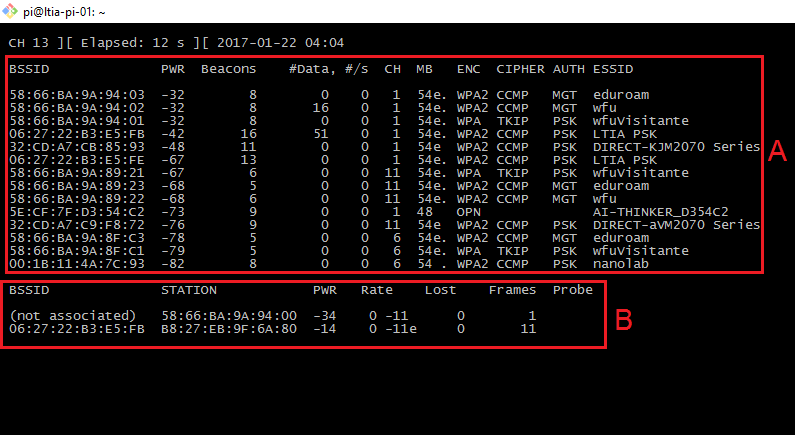
\includegraphics[width=1\textwidth]{040-plataformas/RPi-WiFi-dongles/wifi-sniff-rpi/4-rpi-airodump.png}
	\end{center}
	\nota[Destaque A]{Pacotes do tipo Beacon e suas redes.}
	\nota[Destaque B]{Pacotes entre estações e APs.}
	\legend{Fonte: Elaborada pelo autor}
\end{figure}


Após a avaliação de viabilidade, fez-se necessário o uso de uma aplicação mais
flexível do que o airodump-ng onde fosse possível escolher campos e gerar
relatórios mais flexíveis. Para essa tarefa o software TShark mostrou-se
ideal.

Nele, pode-se escolher, através de argumentos na execução por terminal, a
interface com a opção “-i wlan0”, o modo monitor com opção “-I”, a opção “-T
fields” que altera o funcionamento normal dele para que com as opções “-e
field.field\_child” seja permitido escolher os campos mostrados e juntamente com
as opções “-E separator=, -E quote=d” o formato do relatório gerado torna-se CSV
(\emph{comma separated values} - valores separados por vírgula).

Desta maneira, todos os pacotes capturados são processados pelo TShark e
escritos na saída padrão do terminal (\emph{stdout}), dando a possibilidade de
usar a ferramenta de criação de arquivo, acrescentar em arquivo e redirecionar
para outro processo do terminal Linux (respectivamente ‘>’, ‘»’ e ‘|’). Esta
capacidade, ausente no airodump-ng, é essencial para este trabalho.

Para este trabalho, o comando mais utilizado foi o que mostra os endereços MAC
de origem e transmissão (``wlan.sa'', ``wlan.ta''), os mesmos endereços, porém com nome
de fabricante como prefixo (``wlan.sa\_resolved'', ``wlan.ta\_resolved''), a potência de
sinal (``radiotap.dbm\_antsignal'') e o nome da rede anunciada se o pacote for um
\emph{Beacon}, da mesma maneira que o airodump-ng mostra.

\begin{lstlisting}[language=bash,caption={TShark e opções},label=code-tshark]
pi@sensor-01:~ $ tshark -I -i wlan0 -T fields -E header=y -E quote=d \
-e wlan.sa -e wlan.sa_resolved -e wlan.ta -e wlan.ta_resolved \
-e radiotap.dbm_antsignal -e wlan_mgt.ssid
\end{lstlisting}

Por último, a configuração padrão do TShark não recomenda a execução em modo
supervisor (``root'') por motivo de segurança. Para executá-lo, o usuário precisa ser do
grupo ``wireshark''. Para adicionar o usuário ``pi'' ao grupo ``wireshark'', utiliza-se o comando do
\autoref{code-usermod}.

\begin{lstlisting}[language=bash,caption={Adição do usuário pi ao grupo wireshark},label=code-usermod]
pi@sensor-01:~ $ sudo usermod -a -G wireshark pi
\end{lstlisting}

Este modo de operação permite executar a aplicação final sem necessidade de
elevação de privilégios (\emph{root}), tornando-a mais segura, pois mesmo que
aplicação seja subvertida o sistema operacional não poderá ser comprometido.

\section{Escolha e conclusão}
\label{sec:escolha-plataforma}

Em comparação com o ESP8266, o RPI3 compensou seu custo elevado devido a
facilidade de programação, acesso aos seus recursos e acesso a recursos externos uma
vez que foi possível chegar ao modo promíscuo facilmente através de recursos nativos do
sistema operacional. Para uma comparação das plataformas veja a \autoref{table:comp-hardware-esp-rpi}.

\begin{table}[htb]
\IBGEtab{%
\ABNTEXchapterfont {
	\caption{Comparação das plataformas ESP8266 e RPI3}%
	\label{table:comp-hardware-esp-rpi}
}
}{%
\begin{tabular}{cccc}
\toprule
Aspecto				&	 Raspberry Pi 3 model B					&	ESP-12f		\\
\midrule \midrule
GPIO				&	 27 GPIOs (0 a 26) digitais				&	17 GPIOs digitias e analógicos		\\
\midrule
Número de pinos		&	 40 pinos								&	22 pinos	\\
\midrule
Processamento		&	\emph{ARMv8 64-bit quad-core 1.2 GHz}	&	\emph{Tensilica L106 32-bit (MCU)} com 80		\\
					&	e \emph{VideoCore IV 3D GPU}			&	ou 160 MHz e instruções \emph{16-bit RSIC}	\\
\midrule
Memória RAM			&	  1 GB									&	RAM < 50 kB	\\
\midrule
Memória longo termo	&	 cartão SD (usualmente 8 ou 16 GB)		&	\emph{SPI flash} de 4 MB		\\
\midrule
Tamanho físico		&	 85x56mm								&	 24x13mm	\\
\midrule
Rede embutida		&	 Megabit Ethernet, 802.11 b/g/n			&	802.11 b/g/n	\\
\midrule
Expansão			&	  USB, DSI, CSI e GPIO					&	Somente GPIO	\\
\midrule
Sistema operacional	&	  Qualquer linux/windowns/risc			&	\\
					&	  compilado em ARMv8					&	Não possui	\\
\midrule
Custo				&	 de R\$ 190,00 a R\$ 270,00				&	 de R\$ 12,56 a R\$ 35,87		\\
\midrule
\bottomrule
\end{tabular}%
}{%
	\fonte{Produzido pelo autor.}%
}
\end{table}

O RPI3 foi adotado como plataforma para o sensor de detecção de dispositivos,
pois o modo promíscuo (\emph{monitor mode}) conseguiu ser acessado através de adaptador
USB Wi-Fi. Apesar do esforço para ativação do modo promíscuo na plataforma ESP8266, o uso desta reduziria
significativamente o custo de cada sensor. Para comparação do custo da aplicação
aqui proposta, veja a \autoref{table:comp-app-sensor}.

\begin{table}[ht]
\IBGEtab{%
\ABNTEXchapterfont {
	\caption{Comparação de custos para o sensor da aplicação proposta em função da plataforma}%
	\label{table:comp-app-sensor}
}
}{%
\begin{tabular}{c|cr|cr}
	\toprule
	\multicolumn{5}{c}{Sensor} \\
	\midrule
	Plataforma				&	\multicolumn{2}{|c|}{Raspberry Pi}		&	\multicolumn{2}{|c}{ESP8266}	\\
	\midrule
	Item					&	Descrição			&	Custo em R\$	&	Descrição					&	Custo em R\$	\\
	\midrule
	Plataforma				&	RPI3				&	269,99			&	D1 mini (ESP-12f)			&	12,56	\\
	Fonte de alimentação	&	Fonte Usb iPad		&	13,99			&	Fonte Usb Celular com cabo	&	7,85	\\
												&	Cabo Usb A-micro	&	2,00			&								&		\\
	Adaptador Wi-Fi 		&	Edup Usb			&	16,88			&								&		\\
	Memória			 		&	SD c10 16GB			&	21,99			&								&		\\
	\midrule
	Total por Sensor		&						&	324,85			&								&	20,41	\\
	\midrule\midrule
\end{tabular}%
}{%
	\fonte{Produzido pelo autor.}%
}
\end{table}

É importante notar a proporção de custo entre as duas plataformas onde o RPI3
custa aproximadamente 15 vezes mais por sensor do que a plataforma ESP8266. Isto
justifica o esforço realizado durante o desenvolvimento deste trabalho para
explorar e, com esperança, ativar o modo promíscuo no pequeno dispositivo que
infelizmente não rendeu frutos.

Para a construção do Gateway IoT, as exigências de hardware são
capacidades mínimas de processamento,
armazenamento e comunicação, e a exigência de software é um sistema
operacional que suporte um MQTT Broker. Portanto, para o \emph{gateway}, a
plataforma ESP8266 claramente não é adequada, então um RPI3 representa o custo mínimo.

\begin{table}[ht]
\IBGEtab{%
\ABNTEXchapterfont {
	\caption{Custos para o \emph{gateway} da aplicação proposta}%
	\label{table:custo-app-gw}
}
}{%
\begin{tabular}{c|cr}
	\toprule
	\multicolumn{3}{c}{Gateway}\\
	\midrule
	Item					&	Descrição			&	Custo em R\$	\\
	\midrule
	Plataforma				&	RPI3				&	269,99			\\
	Fonte de alimentação	&	Fonte Usb iPad		&	13,99			\\
												&	Cabo Usb A-micro	&	2,00			\\
	Memória			 		&	SD c10 16GB			&	21,99			\\
	\midrule
	Total por Gateway		&						&	307,97			\\
	\midrule
	\bottomrule
\end{tabular}%
}{%
	\fonte{Produzido pelo autor.}%
}
\end{table}


\chapter{Aplicação demonstrativa}
\label{chap:aplicacao_demonstrativa}

Para a construção do software aplicativo, foi utilizado uma arquitetura em
três camadas: sensor, distribuidor de acesso (\emph{IoT gateway}) e apresentação
(Web). Nesta divisão, os sensores capturam as informações dos dispositivos
e repassam para a camada seguinte, no \emph{gateway} todas as partes se
encontram para fornecer e solicitar informações e, por último, a camada de
apresentação coleta o que é enviado dos sensores e gera uma página Web
para visualização dos dados capturados.

Esta divisão está de acordo com o padrão encontrado em outras aplicações
IoT onde a última camada usualmente varia entre apresentação e mineração
de dados (\emph{Data Mining}).

A camada de sensor utilizou as tecnologias Node.js, TShark parte
do Wireshark e MQTT.js. A camada \emph{gateway} foi composta
basicamente pelo \emph{MQTT Broker} Mosquitto. Por fim a camada de
apresentação utlizou as tecnologias Node.js, MQTT.js, HTML,
CSS, Javascript, Bootstrap e Google Maps API. A \autoref{fig-arq-app} apresenta
a arquitetura geral da aplicação demonstrativa.

\begin{figure}[htb]
	\caption{\label{fig-arq-app}Arquitetura geral da aplicação demonstrativa}
	\begin{center}
		\includegraphics[width=1\textwidth]{050-construcao/esquema-proj.png}
	\end{center}
	\legend{Fonte: Elaborada pelo autor}
\end{figure}


\chapter{Resultados e Discussão}
\label{chap:resultados}

Neste capítulo, são abordados, analisados e discutidos os resultados encontrados
durante a exploração do tema e das plataformas e durante a implementação das
aplicações, além de verificar a precisão atingida com a aplicação implementada.
Todos os testes foram realizados no prédio do laboratório LTIA da Unesp de
Bauru, onde os sensores permaneceram monitorando dispositivos.

\section{Método de teste}
\label{sec:metodo-teste}

Como discutido no \autoref{chap:aplicacao_demonstrativa}, a arquitetura geral da
aplicação (\autoref{fig-arq-app}) mostra que a precisão vista na aplicação Web
depende dos resultados encontrados pela aplicação sensor que, por sua vez,
depende do par de capacidades combinadas do hardware adaptador Wi-Fi e do
software TShark. Portanto, a metodologia de testes empregada neste capítulo é
analisar diretamente as capacidades deste último par. Esta decisão também se
deve pela facilidade de armazenar e analisar arquivos CSV gerados pelo TShark.

As capturas foram executadas com o comando descrito no
\autoref{code-tshark-pipe-assinc} que é o mesmo utilizado na aplicação sensor.

\begin{lstlisting}[language=bash,caption={TShark e redirecionamento da saída para arquivo assíncrono},label=code-tshark-pipe-assinc]
pi@sensor-01:~ $ tshark -I -i wlan0 -T fields -E header=y -E quote=d \
-e wlan.sa -e wlan.sa_resolved -e wlan.ta -e wlan.ta_resolved \
-e radiotap.dbm_antsignal -e wlan_mgt.ssid \
>> 2017-01-17--02-48--rpi-02.csv &
pi@sensor-01:~ $
\end{lstlisting}

Neste modo de uso, os resultados são direcionadas para a saída padrão (stdout)
do terminal e podem ser capturados por outro programa no formato de valores
separados por vírgula (CSV). Os campos escolhidos para captura são
\texttt{``wlan.sa''}, \texttt{``wlan.sa\_resolved''}, \texttt{``wlan.ta''},
\texttt{``wlan.ta\_resolved''}, \texttt{``radiotap.dbm\_antsignal''} e
\texttt{``wlan\_mgt.ssid''}.

Na linha 4 do \autoref{code-tshark-pipe-assinc}, o \texttt{``\&''} representa o início
de um processo independente (assíncrono) e, a linha 5, a finalização do terminal.
Esta operação foi somente executada durante a captura longa.

A análise de dados foi feita com a função \texttt{``summary''} da ferramenta
``Ron’s editor''\footnote{\url{https://www.ronsplace.eu/Products/RonsEditor}}
e a filtragem com a função \texttt{``Filter''} da ferramenta
``RecCsvEditor''\footnote{\url{http://recsveditor.sourceforge.net/}}. Para a
construção dos gráficos, foi utilizada a ferramenta
``WPS Spreadsheets''\footnote{\url{https://www.wps.com/office-free}}.


\chapter{Conclusão}
\label{chap:Conclusao}


Esse projeto teve como objetivo o aprofundamento na área de Internet das Coisas,
especialmente nas características de desenvolvimento local e independente que
foram encontradas durante a construção da aplicação localizadora de contexto de
dispositivos. Esta aplicação foi construída, instalada e testada no prédio
piloto fornecendo um ambiente real onde pôde-se avaliar as reais capacidades de
um sistema localizador desse gênero.

Confirmou-se que um sistema de
geolocalização que utiliza somente FSPL com RSS tem poucas chances de ser
preciso. Porém, com as mesmas ferramentas, pôde-se construir uma rede de sensores
onde cada nó foi responsável por monitorar um contexto (sala, área ou parte de um
prédio) e, neste sentido, os dispositivos puderam ser associados ao contexto e a
localização do sensor, efetivamente identificando a localização deles
e seus portadores dentro de um modelo lógico do prédio.

Para que a implementação possa ser replicada, o custo associado foi determinado
como sendo de R\$ 324,85 por sensor onde é necessário um sensor por contexto além
de uma estrutura de rede já existente. Analogamente, o custo total do projeto
piloto foi definido como R\$ 995\footnote{Valor total das aquisições no
MercadoLivre.com} para os custos de hardware incluindo os protótipos e 400
horas\footnote{Estimado de 200 funcionalidades (\emph{git commit}) implementadas
com média de 2 horas de implementação cada} de desenvolvimento para o software e
documentação.

Quanto ao estado da arte do ramo de Internet das Coisas foram identificadas
algumas características que necessitam destaque:

\begin{alineas}
	\item Num ambiente onde
	idealmente todos os objetos e coisas estão conectados, poucos padrões globais
	existem para garantir essa conexão, tanto a nível jurídico (direitos e
	obrigações de fabricantes, desenvolvedores e usuários) quanto técnico
	(protocolos de comunicação, arquiteturas e recomendações unificados);

	\item Muitos produtos e soluções são muito jovens e carecem amadurecimento,
	especialmente no mercado residencial e comercial, onde as exigências de
	segurança, padronização, conformidade legal e disponibilidade são inferiores
	às encontradas no ramo industrial;

	\item Foi encontrada uma dificuldade durante a aquisição das plataformas, pois
	sem uma orientação de um profissional da área de sistemas embarcados, a
	comparação e escolha de uma plataforma é uma tarefa muito complexa;

	\item Comparada com a comunidade de desenvolvedores Web, a comunidade
	de desenvolvedores IoT é muito jovem e não desenvolveu ferramentas para
	construir, compartilhar e reutilizar projetos de maneira eficiente.
\end{alineas}


\section{Resultados para comunidade e trabalhos futuros}
\label{sec:trab-futuros}

Durante a exploração do tema, foram encontradas diversas implementações de
localizadores baseados em Wi-Fi, mas a implementação aqui executada mais se
assemelha com a de \citeonline{Ferreira2016} onde a mesma plataforma
(Raspberry Pi, porém na sua versão 2 modelo B+), tipo de adaptador (Wi-Fi USB)
e software (TShark) foram utilizadas. A principal diferença são os
objetivos, enquanto a localização que \citeonline{Ferreira2016} buscou é do tipo
geográfica, neste trabalho buscou-se o objetivo mais simples de encontrar o grau
de presença do dispositivo no mesmo contexto (sala) do sensor. Outras diferenças
são que alguns desafios propostos por \citeonline{Ferreira2016} foram atacados
com certo nível de sucesso, entre eles: mais de um dispositivo sensor,
coleta e processamento simultâneos (\emph{online}) e registro do histórico.
Outros que não renderam frutos também merecem atenção, como a exploração
adicional da plataforma ESP8266 que aqui propõem-se como trabalho futuro para a
construção do mesmo sensor a um menor custo.


% ----------------------------------------------------------
% ELEMENTOS PÓS-TEXTUAIS
% ----------------------------------------------------------
\postextual
% ----------------------------------------------------------

% ----------------------------------------------------------
% Referências bibliográficas
% ----------------------------------------------------------
% \bibliography{900-referencias/referencias}
\bibliography{900-referencias/TCC-intro,900-referencias/TCC-problema,900-referencias/TCC-teorica,900-referencias/TCC-teorica-redes,900-referencias/TCC-teorica-iot,900-referencias/TCC-teorica-contexto,900-referencias/TCC-metodo,900-referencias/TCC-plataformas}

% ----------------------------------------------------------
% Glossário
% ----------------------------------------------------------
% Consulte o manual da classe abntex2 para orientações sobre o glossário.
\ifglossario
	Glossário
\fi

% ----------------------------------------------------------
% Apêndices
% ----------------------------------------------------------
\ifapendice
	% Inicia os apêndices
	\begin{apendicesenv}

	% Imprime uma página indicando o início dos apêndices
	\partapendices

	% ----------------------------------------------------------
	\chapter{Compras Mercado Livre}

	\includegraphics[scale=1.1]{920-apendices/Compras-MercadoLivre.pdf}
	\includegraphics[scale=1.1,page=2]{920-apendices/Compras-MercadoLivre.pdf}

	% ----------------------------------------------------------
	\end{apendicesenv}
\fi
% ---
\ifanexo
	Anexo de outros autores.
\fi

\ifindice
	Indice Remissivo
\fi

\end{document}
